\documentclass[convert={density=300,outext=.png}]{standalone}
\usepackage{tikz}

\begin{document}
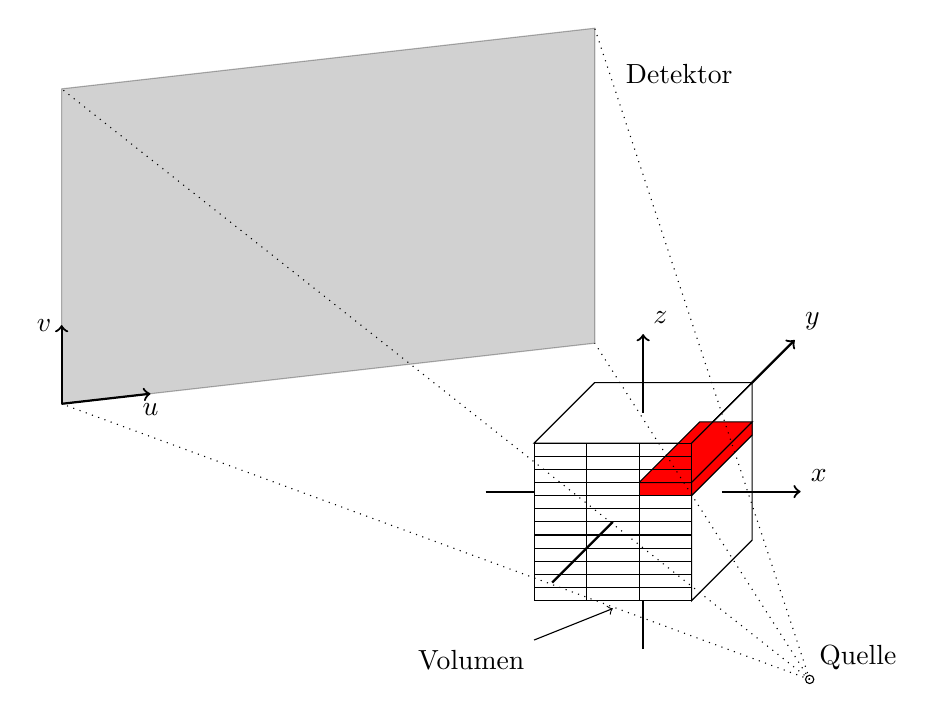
\begin{tikzpicture}[axis/.style={thick,->}]
    \draw[fill=black!60!white,opacity=0.3] (0, 0, 0) -- (0, 4, 0) -- (6, 4, -2) -- (6, 0, -2) -- (0, 0, 0);
    \draw[axis] (0, 0, 0) -- (0, 1, 0) node[left] {$v$};
    \draw[axis] (0, 0, 0) -- (1, 0, -0.33333333) node[below] {$u$};

    % Achsenanfang
    \draw[thick] (5, -1.5, -1) -- (6, -1.5, -1); % x
    \draw[axis] (7, -1.5, -2) -- (7, -1.5, -6) node[above right] {$y$}; % y
    \draw[thick] (7, -3.5, -1) -- (7, -2.5, -1); % z

    % Volumen
    \draw[fill=white] (6, -0.5, -2) -- (8, -0.5, -2) -- (8, -0.5, 0) -- (6, -0.5, 0) -- (6, -0.5, -2);
    \draw[fill=white] (6, -0.5, 0) -- (8, -0.5, 0) -- (8, -2.5, 0) -- (6, -2.5, 0) -- (6, -0.5, 0);
    \draw[fill=white] (8, -0.5, -2) -- (8, -2.5, -2) -- (8, -2.5, 0) -- (8, -0.5, 0) -- (8, -0.5, -2);

    \draw[->] (6, -3, 0) -- (7, -2.6, 0) node[pos=0,below left] {Volumen};

    % Achsenende
    \draw[axis] (8, -1.5, -1) -- (9, -1.5, -1) node[above right] {$x$}; % x
    \draw[thick] (7, -1.5, 2) -- (7, -1.5, 0); % y
    \draw[axis] (7, -0.5, -1) -- (7, 0.5, -1) node[above right] {$z$}; % z

    % Teilvolumen
    \draw[fill=red] (7.333333, -1, 0) -- (8, -1, 0) -- (8, -1.166666, 0) -- (7.333333, -1.166666, 0)
                    -- (7.333333, -1, 0);
    \draw[fill=red] (7.333333, -1, 0) -- (7.333333, -1, -2) -- (8, -1, -2) -- (8, -1, 0) -- (7.333333, -1, 0);
    \draw[fill=red] (8, -1, 0) -- (8, -1, -2) -- (8, -1.166666, -2) -- (8, -1.166666, 0) -- (8, -1, 0);

    \draw (6.666666, -0.5, 0) -- (6.666666, -2.5, 0); % v1
    \draw (7.333333, -0.5, 0) -- (7.333333, -2.5, 0); % v2
    \draw (6, -0.666666, 0) -- (8, -0.666666, 0); % h1
    \draw (6, -0.833333, 0) -- (8, -0.833333, 0); % h2
    \draw (6, -1, 0) -- (8, -1, 0); % h3
    \draw (6, -1.166666, 0) -- (8, -1.166666, 0); % h4
    \draw (6, -1.333333, 0) -- (8, -1.333333, 0); % h5
    \draw (6, -1.5, 0) -- (8, -1.5, 0); % h6
    \draw (6, -1.666666, 0) -- (8, -1.666666, 0); % h7
    \draw (6, -1.833333, 0) -- (8, -1.833333, 0); % h8
    \draw (6, -2, 0) -- (8, -2, 0); % h9
    \draw (6, -2.166666, 0) -- (8, -2.166666, 0); % h10
    \draw (6, -2.333333, 0) -- (8, -2.333333, 0); % h11

    % fehlende Linien nachzeichnen
    \draw (8, -0.5, 0) -- (8, -0.5, -2);
    \draw (8, -0.5, 0) -- (8, -2.5, 0);
    \draw (6, -0.5, 0) -- (8, -0.5, 0);

    % Quelle und Kegelstrahl
    \coordinate (s) at (9.5, -3.5, 0);
    \draw (s) circle (1.5pt) node[above right] {Quelle};
    \draw[dotted] (s) -- (0, 0, 0);
    \draw[dotted] (s) -- (0, 4, 0);
    \draw[dotted] (s) -- (6, 4, -2) node[pos=0.9,above right] {Detektor};
    \draw[dotted] (s) -- (6, 0, -2);
\end{tikzpicture}
\end{document}
